%----------------------------------------------------------------------------
\chapter{\AudioOverIp}
%----------------------------------------------------------------------------
\section{Bevezetés az Audio over IP világába}
%----------------------------------------------------------------------------
Az 1990-es évek végén a professzionális hangtechnika fokozatosan elmozdult a hagyományos pont-pont 
digitális átviteli rendszerekről (mint az AES/EBU vagy MADI) az IP-alapú megoldások irányába, például az AES67 szabvány felé. 
Ez az új, csomagalapú hálózati technológia jelentős rugalmasságot hozott a hangrendszerek terén, valamint lehetőséget adott 
a vezérlés és monitorozás bővítésére. Ennek köszönhetően a meglévő telepítések könnyen bővíthetők és frissíthetők szoftveres 
konfigurációk révén, így a rendszer idővel további funkciókkal gazdagodhat, anélkül, hogy fizikai módosításokat kellene végezni.

Az IP-alapú rendszerek egyik legnagyobb előnye, hogy a jelutak már nem kötődnek egy-egy fizikai kábelhez, 
ami azt jelenti, hogy néhány kattintással megváltoztathatók a hálózati beállítások anélkül, hogy fizikai 
átrendezésekre vagy dedikált audioroute hardverekre lenne szükség. A csomagokba szervezett adatátvitel 
lehetővé teszi, hogy az audiojelek automatikusan elérjenek a kívánt célállomásokhoz az IT hálózaton keresztül.

A CobraNet, amelyet a Cirrus Logic 1996-ban vezetett be, az első széles körben használt audio-over-ethernet 
technológiának tekinthető. Ezt a rendszert számos helyen alkalmazzák, mint például kongresszusi 
központokban, színházakban, koncerttermekben, repülőtereken és vidámparkokban. 
Noha a CobraNet még mindig megtalálható bizonyos telepítésekben, magas késleltetése és 
korlátozott skálázhatósága miatt nem ideális élő hangosítási rendszerekhez, stúdiófelvételekhez vagy rádiós alkalmazásokhoz.

A 2000-es évek közepén jelent meg az Audinate által kifejlesztett Dante rendszer, amely a `Digital Audio Network Through Ethernet' rövidítése. 
A Dante jelentős előrelépést hozott a korábbi audio-over-IP technológiákhoz képest, különösen a 
használhatóság és a szabványos hálózati infrastruktúrával való kompatibilitás terén. 
A Dante nagy előnye a széleskörű hardveres ökoszisztémája, amely több száz gyártó által gyártott több ezer eszközzel működik együtt.

Mielőtt a Dante elérte volna piacvezető pozícióját, az AVB (Audio Video Bridging) technológia is 
nagy figyelmet kapott. Bár az AVB eredetileg a hang- és videóalkalmazásokhoz készült, 
más iparágak, például az autóipar és az ipari automatizálás is átvették ezt a technológiát, 
és egy általánosabb nevet kapott: TSN (Time Sensitive Network), amely az időérzékeny hálózatokat fedi le.

A Milan munkacsoport, amely audio- és videorendszerek gyártóiból áll, 
finomhangolt specifikációt dolgozott ki a professzionális audio- és videorendszerek számára, 
amelyet Milan néven ismerhetünk. Ez a specifikáció egy TSN-alapú verzió, amelynek fő célja az 
interoperabilitás biztosítása a különböző audio- és videorendszerek között.

%----------------------------------------------------------------------------

Az IP-alapú hálózatokra való átállás hasonló folyamatként írható le, mint amikor az analóg hangtechnikáról áttértek
a digitális megoldásokra. Kezdetben csak néhány úttörő telepítés használja az új technológiát, 
és ezek kezdetben kezelési vagy megbízhatósági problémákat mutathatnak a hagyományos rendszerekkel szemben. 
Azonban, ahogy a technológia fejlődik, ezek a hiányosságok fokozatosan megszűnnek.

Az IT-alapú hálózatok bizonyos szempontból alapvetően eltérnek a hagyományos audió útvonalaktól. 
Először is, a szokásos IT hálózatok nem feltétlenül felelnek meg az audió rendszerekre jellemző 
szigorú időzítési követelményeknek. A hálózati csomagok továbbítása során egyes csomagokat más, 
párhuzamosan haladó csomagok késleltethetnek, ami az audióadatok esetében hallható időbeli eltérésekhez vezethet. 
Ezzel szemben a hagyományos audiókábelek használata esetén a továbbítási időzítés stabil és állandó marad.

Továbbá, az IT-alkalmazások esetében a csomagvesztés nem jelent komoly problémát, mivel az elveszett 
adatokat a rendszer automatikusan újraküldi. Az audió alkalmazásoknál viszont kulcsfontosságú, hogy 
a csomagok már az első alkalommal hibamentesen megérkezzenek, mivel az újraküldésre nincs elegendő idő. 
Egy-egy elveszett csomag azonnal hallható zavarokat, megszakításokat okozhat az audiófolyamban.

A csomagvesztés gyakori oka lehet a hálózati linkek túlterheltsége vagy a túl kicsi pufferméret. 
Ezért az audióhálózatok tervezésekor ügyelni kell arra, hogy minden felhasználó számára elegendő 
sávszélesség álljon rendelkezésre, még teljes terhelés mellett is. Amennyiben biztosítva van az 
adatcsomagok időben történő továbbítása, a hálózat stabil és hosszú távon megbízhatóan működhet. 
Ugyanakkor érdemes a hálózatot megfelelő mértékben túlméretezni annak érdekében, hogy minden csomag 
időben célba érjen, anélkül, hogy a kapcsolók bonyolult finomhangolására lenne szükség.

Ez azt jelenti, hogy olyan IT-hálózatokat kell kiépíteni, amelyek dedikált sávszélességet 
biztosítanak az audió alkalmazások számára, és elkerülik az egyéb, általános célú alkalmazásokkal való közös használatot.

%----------------------------------------------------------------------------

Az audio-over-IP technológiák többsége azon a feltételezésen alapul, hogy az alapjául szolgáló hálózat megbízhatóan üzemel, 
tehát nem fordul elő csomagvesztés, és a csomagok nem ütköznek jelentős mértékben más adatforgalommal a hálózati kapcsoló eszközökön. 
Azonban bizonyos hálózatok esetében, különösen ha az audióadatokat más típusú forgalommal, például általános 
internetes forgalommal vegyítik, kulcsfontosságú lehet, hogy az audió- és szinkronizációs csomagok elsőbbséget 
élvezzenek más típusú adatátvitelhez képest, például a webes böngészéshez viszonyítva. Szerencsére a mai, kereskedelmi 
forgalomban kapható kapcsolók többsége képes ilyen típusú prioritás beállítására, így biztosítható az audiórendszerek zavartalan működése. \newline

Példa audio over IP hálózatokra:
%----------------------------------------------------------------------------
\begin{itemize}
	\item Audinate által kifejlesztett - Dante
\end{itemize}
\begin{itemize}
	\item QSC által kifejlesztett - Q-LAN
\end{itemize}
\begin{itemize}
	\item Lawo és Partnerei által kifejlesztett - RAVENNA
\end{itemize}
%----------------------------------------------------------------------------
\begin{figure}[H]
	\centering
	
\includegraphics[width=50mm, keepaspectratio]{figures/dante_logo.jpg}
	\caption{Audinate Dante logó}
	\label {fig:dante_logo}
\end{figure}
%----------------------------------------------------------------------------
\subsection{Előnyök és hátrányok}
%----------------------------------------------------------------------------
Az IT hálózatok alkalmazása hangkapcsolatokra nézve számos előnyt kínál:
\begin{itemize}
	\item Rugalmasság hangkapcsolatok hozzáadásához vagy módosításához anélkül,
	      hogy kábeleket cserélnénk.
\end{itemize}
\begin{itemize}
	\item Viszonylag alacsony áron széles skálájú funkciókat kínál.
\end{itemize}
\begin{itemize}
	\item Alkalmazkodás és integráció az IT hálózati infrastruktúrákba
	      specifikus audio vagy videokábelek alkalmazása nélkül.
\end{itemize}
\begin{itemize}
	\item Videójel és vezérlési adatok továbbíthatók ugyanazon infrastruktúrán
	      keresztül.
\end{itemize}
%----------------------------------------------------------------------------
Ugyanakkor az audio-over-IP hálózatok felhasználóit számos kihívás elé is állíthatják:
%----------------------------------------------------------------------------
\begin{itemize}
	\item Azért mert általában több hangmintát egy csatornából egy csomagba helyeznek
	      el a hatékonyság érdekében, adott minimális késleltetés adódik, mivel az
	      küldőnek meg kell várnia, hogy a hangminták rendelkezésre álljanak, mielőtt
	      azokat átküldené a hálózaton. Ez a késleltetés általában magasabb, mint a
	      pont-pont digitális hangszabványok esetében, de optimalizált csomagformátumok és
	      hálózati beállítások segítségével minimalizálható és nagyon jól közelíthető.
\end{itemize}
\begin{itemize}
	\item Mivel az IT hálózatok nem meghatározottak a csomagok út idejét tekintve,
	      egy biztonsági tartományt, azaz egy audio buffer-t kell beszúrni a fogadó végén.
	      Ez a buffer további késleltetést eredményez. Minél kevesebb csomagütközés van
	      jelen a hálózatban, annál inkább csökkenthető ez a biztonsági tartomány és
	      ezzel a késleltetés.
\end{itemize}
\begin{itemize}
	\item Az audio csomagformátumok változatossága miatt növekszik a komplexitás,
	      ami azt jelenti, hogy a fogadóknak és küldőknek azonos beállításokkal kell
	      rendelkezniük. Az audio-over-IP technológia komplexitása jelentősen magasabb,
	      mint az előző technológiáké. Az iparág még mindig jelentős munkát végez annak
	      érdekében, hogy csökkentse ezt a komplexitást a felhasználók számára, bevezetve
	      intelligens és felhasználóbarát szoftvermegoldásokat az audiohálózatok
	      kezelésére.
\end{itemize}
%----------------------------------------------------------------------------
\subsection{Fázishelyesség}
%----------------------------------------------------------------------------
Az audioalkalmazások többségénél alapvető fontosságú a különböző eszközök szinkronizált működése. 
Különösen lényeges a mikrofonok és hangszórók közötti fázishelyesség biztosítása. 
Ha egy erősítőhöz több hangszóró csatlakozik, és az összes csatorna adata egyetlen hangcsomagban érkezik meg, 
nem áll fenn annak a veszélye, hogy a csatornák fáziskéséssel működnének, mivel az audio minták a 
hálózati átvitel során nem torzulhatnak egymáshoz képest.

Ezzel szemben, számos olyan alkalmazás létezik, ahol több erősítő és processzor egymástól függetlenül 
kapja a hangcsomagokat, ugyanakkor továbbra is szükséges, hogy az audiojelek fázishelyesen legyenek reprodukálva. 
Ilyen esetekben ugyanazt a hangcsomagot több hálózati eszköz is megkapja és puffereli, és ezeket a jeleket 
pontosan ugyanabban az időpontban kell lejátszaniuk, hogy elkerüljék az időzítési eltéréseket.

Mivel az IT-hálózatokban nincsenek szigorúan meghatározott időzítési előírások a csomagok továbbítási és 
érkezési idejére, az audió hálózatokban külön szinkronizációs mechanizmusra van szükség. 
Ez egy jelentős kihívás, amelyet minden audio-over-IP technológiának meg kell oldania.

A szinkronizációt az audió hálózatokon belül a Precision Time Protocol (PTP) segítségével valósítják meg, 
amely biztosítja, hogy az összes eszköz pontosan szinkronban legyen. 
Ennek értelmében minden hálózati eszköz belső órája (PTP követő) egy központi referenciaórához (PTP vezető) igazodik. 
A PTP vezető szerepét bármely olyan audióeszköz betöltheti, amely alkalmas erre a feladatra, vagy egy 
speciálisan erre a célra fejlesztett eszköz, amely pontos időreferenciát szolgáltat. 
A vezetőt vagy manuálisan választják ki, vagy egy szabványos automatikus mechanizmus alapján történik a kiválasztás.

Az audio adók és vevők számára az alapvető követelmény az, hogy pontosan ehhez az időreferenciához szinkronizáljanak. 
Amikor egy audio csomagot elküldenek, időbélyeggel látják el, amely a küldési időt jelöli. 
A vevőkben egy előre meghatározott időeltolást, úgynevezett linkeltolást állítanak be, amely biztosítja a 
megfelelő pufferelést és a zökkenőmentes lejátszást. Így a hang lejátszása akkor történik, amikor a küldési 
idő és a linkeltolás összeadódik, biztosítva ezzel a pontos időzítést. \newline

Minden vevő két feltétel mellett érheti el egymás között a fázispontosságot:
%----------------------------------------------------------------------------
\begin{itemize}
	\item Pontos időszinkronizálás a PTP óra vezetőjéhez (azonos időbázis).
	\item Azonos linkeltolási érték beállítása a felhasználó által az összes vevőeszközön.
\end{itemize}
%----------------------------------------------------------------------------
Az audiohálózatokban alkalmazott linkeltolást mindig a legnagyobb várható késleltetés alapján kell 
beállítani az összes érintett kapcsolat esetében. Fontos, hogy némi tartalékot is hozzárendeljünk a 
beállított értékhez, amely lehetővé teszi az esetleges, váratlan csomagkiszállítási időingadozások kezelését. 
Ez azt jelenti, hogy a feldolgozási idő átlagánál valamivel hosszabb időkeretet hagyunk. 
Szerencsére ez a megközelítés már széles körben elterjedt, és minden modern audiohálózati szabványban alkalmazásra került.
%----------------------------------------------------------------------------
\begin{figure}[H]
	\centering
	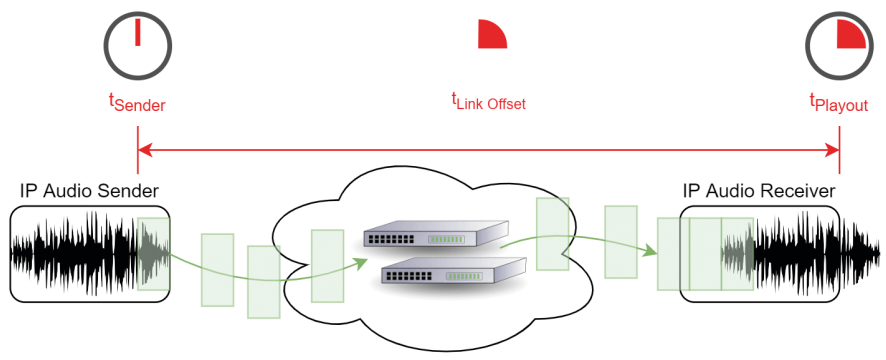
\includegraphics[width=\linewidth, keepaspectratio]{figures/link_offset_latency.png}
	\caption{A kapcsolati eltolás meghatározza a késleltetést \cite{AHNERT2023}}
	\label {fig:link_offset_latency}
\end{figure}
%----------------------------------------------------------------------------
\begin{figure}[H]
	\centering
	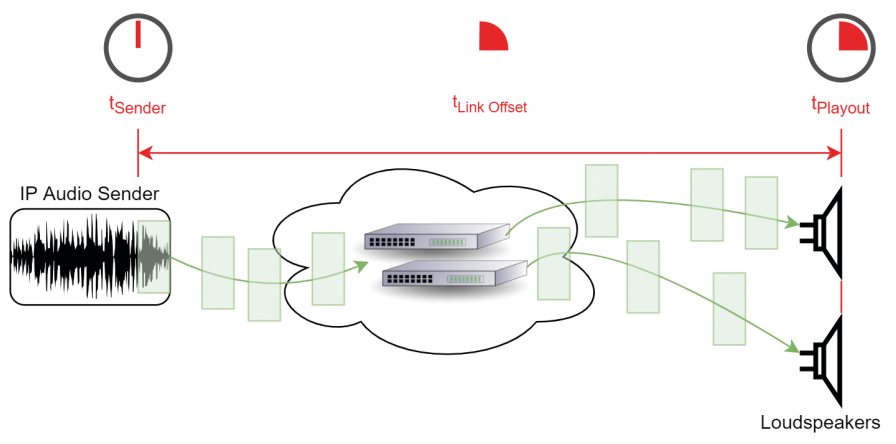
\includegraphics[width=\linewidth, keepaspectratio]{figures/phase_coherence_link_offset.png}
	\caption{Fáziskoherencia azonos kapcsolati eltolással \cite{AHNERT2023}}
	\label {fig:phase_coherence_link_offset}
\end{figure}
%----------------------------------------------------------------------------
\subsection{Szinkronizáció}
%----------------------------------------------------------------------------
Az audiohálózatokban alkalmazott linkeltolást mindig a legnagyobb várható késleltetés alapján 
kell beállítani az összes érintett kapcsolat esetében. Fontos, hogy némi tartalékot is 
hozzárendeljünk a beállított értékhez, amely lehetővé teszi az esetleges, váratlan csomagkiszállítási időingadozások kezelését. 
Ez azt jelenti, hogy a feldolgozási idő átlagánál valamivel hosszabb időkeretet hagyunk. 
Szerencsére ez a megközelítés már széles körben elterjedt, és minden modern audiohálózati szabványban alkalmazásra került.

Az IP alapú küldők és vevők precíz szinkronizációja kulcsfontosságú a minimális késleltetéssel történő működés érdekében. 
A hagyományos audioeszközök esetében ez a szinkronizáció jellemzően különálló word clock kapcsolaton keresztül, 
vagy szinkronizált audioformátumok, például AES/EBU vagy MADI segítségével történt. Ezek a rendszerek egyértelmű 
jelet biztosítottak a mintavételi időpontra vonatkozóan, amely lehetővé tette a vevők számára a frekvencia és 
fázis pontos kinyerését, például analóg-digitális átalakítók esetében.

A PTP (Precision Time Protocol) csomagok kis méretűek, így nem terhelik jelentősen a hálózatot, azonban 
elengedhetetlen, hogy a hálózati eszközökben kiemelt prioritással kerüljenek továbbításra. 
Ez hozzájárul a szinkronizációs pontosság javításához. A QoS (Quality of Service) szabályok keretein belül a 
PTP csomagoknak még magasabb prioritást kell kapniuk, mint a hangátvitel során használt csomagoknak, hogy 
biztosítsák a pontos időzítést az egész hálózatban.

Az összes hálózati eszköz a PTP segítségével egyetlen referenciaidőponthoz igazodik. Ezt az időt egy 
úgynevezett óravezető (PTP leader) eszköz határozza meg, míg a többi eszköz óra követőként szinkronizálódik hozzá. 
Minden eszköz ebből az abszolút időből generálja a saját belső óráját, amit médiaórának nevezünk. 
A gyártóknak gondoskodniuk kell arról, hogy a médiaóra frekvenciája és fázisa pontosan megegyezzen minden eszköz 
esetében, amely a hálózatban működik. Bár technikailag elérhető a magas fokú pontosság, ennek megvalósítása jelentős kihívást 
jelent az audioeszközöket gyártó vállalatok számára. 
A szinkronizáció minősége eszközönként változhat, azonban elfogadhatónak tekinthető, ha a fáziskésés mértéke nem haladja meg az 1 mikroszekundumot.

Mivel az IT-hálózatok nem determinisztikusak a csomagok érkezési idejének tekintetében, az eszközök pontos
szinkronizálása összetett megoldásokat követel meg. 
A PTP követők fő feladata két hatás kompenzálása, amelyek bármilyen hálózat esetén előfordulhatnak:
%----------------------------------------------------------------------------
\subsubsection{Jitter kompenzáció}
%----------------------------------------------------------------------------
A PTP vezető által küldött szinkronizációs üzenetekben szereplő aktuális időt minden követő eszköz 
megkapja egy ismert multicast cím (224.0.1.129) segítségével. A hálózati infrastruktúra és a 
kapcsolók sajátosságai miatt azonban ez az információ nem mindig érkezik meg egyenletes késleltetéssel a vevőkhöz. 
A késleltetés ingadozása a csomag jitter, illetve csomag késleltetési változás (Packet Delay Variation, PDV) 
nevű jelenség, amelyet minden PTP követőnek képesnek kell lennie kompenzálni. 
Az ilyen típusú hálózatokban az audioeszközök jellemzően 1–8 szinkronizációs üzenetet dolgoznak fel másodpercenként, 
ahol a 8-as érték az interoperabilitás biztosítása érdekében van ajánlva.




% 🚩✋🏻🛑⛔️




%----------------------------------------------------------------------------
\subsubsection{Késleltetés mérése}
%----------------------------------------------------------------------------
A követő második kulcsfontosságú feladata a vezető és a követő közötti
csomagkésleltetés mérése a vezető által szinkronizációs üzenetekben kapott
idő kijavításához. Ehhez szükség van arra az időmérésre, amelyek azt mutatja meg számunkra,
hogy a hálózati út során mennyi időbe telik egy csomag átvitele.
Ez a mérés magában foglalja az összes közöttük lévő
összetevő késleltetését, beleértve a kábeleket és kapcsolókat is. 
A vezető és a követő közötti kábelhossz és a kapcsolók száma nem számít, csak a végső érték.
A PTP időnek az összes követő között ugyanannak kell lennie nanoszekundum pontossággal.

Az egyetlen feltétel a PTP számára, hogy a késleltetés mindkét irányban, a vezetőtől a
követőig és fordítva, állandó és szimmetrikus maradjon.
A késleltetést a követő két üzenet cseréjével méri, a késleltetési kérésből és a késleltetési válaszból következően.
Ezt a késleltetést általában a szinkronizálási aránnyal azonos gyakorisággal hajtják végre.
%----------------------------------------------------------------------------
Mivel a hálózaton több eszköz is képes lehet PTP vezetőként működni,
a szabvány szabályokat hozott létre a vezető
kiválasztásához. Ezt a szabályt a Best Master Clock Algorithm (BMCA), vagyis a
Legjobb Mesteróra Algoritmusnak nevezik. 

Minden vezetőképes eszköz küldhet bejelentő üzeneteket a prioritásairól,
valamint az oszcillátor pontosságáról. Ezenkívül figyelnie kell más eszközöket,
amelyek szintén elküldhetik saját bejelentő üzeneteiket. 
Ha más bejövő üzenetek jobb minőséget jelentenek, az eszköz leállítja a vezetőként való bejelentkezését.
Ellenkező esetben rendszeresen küldi saját üzeneteit, mintegy \textit{szívverésként},
és ezzel jelezve minden másik eszköznek az aktív állapotát. 

Ezeket az üzeneteket az announce intervallumnak nevezett időközönként küldik el. 
A bejelentő üzenetek szolgálnak \textit{szívverésként} is, hogy mások tudják, a jelenlegi mester még működőképes.
Ha a kapcsolat megszakad, az összes egység vár egy bizonyos időt (bejelentő időtúllépés),
amíg elküldik bejelentő üzeneteiket, majd megismétlik a kiválasztási folyamatot. 
A vezetőváltás idején a követőknek folytatniuk kell saját oszcillátoruk belső működését.
Az audio nem szakítható meg a vezetőváltás során.
A bejelentő üzenetekben megadott minőség két értéket tartalmaz, amelyeket a felhasználó állít be: prioritás 1 és prioritás 2.
Mindkettő értéke 0 és 255 között változhat, ahol a 0 érték a legjobb és legyőzi a többieket.
Ha egy prioritás 1 érték kisebb egy eszközön, mint más eszközökön,
akkor az lesz a vezető. A prioritás 2 alatti érték csak akkor releváns, ha
minden előző érték, beleértve a prioritás 1-et is, több eszközön ugyanaz. 
Ez előfordulhat két azonos típusú eszköz telepítéseknél, amelyeknek a felhasználó
azonos értéket állított be a prioritás 1-hez. Ebben az esetben a prioritás 2
határozza meg, hogy melyik lesz a fő vezető, és melyik a tartalék. 

Fontos megjegyezni, hogy néhány eszköz nem kínál lehetőséget a felhasználónak ezen értékének megadására.
Ehelyett egyszerűen a \textit{Preferált Vezető} megjelölésével rendelkeznek.
Technikailag ezek a termékek rögzített értéket használnak bejelentő üzeneteikben, amit a gyártó határoz meg.
Ezért még mindig lehetséges, hogy egy másik PTP vezetőnél beírva egy még alacsonyabb értéket, felül bírálhatja az ilyen típusú eszközt.
Néhány támogatja azt a beállítást is, amit \textit{Csak Követő} néven ismerünk. Ebben az esetben amikor ez engedélyezve van,
az adott eszköz sosem próbálja meg átvenni a vezetői szerepet az PTP hálózaton.
%----------------------------------------------------------------------------
\subsection{Mintavételi frekvencia és bitmélység}
%----------------------------------------------------------------------------
Az audio over IP rendszereknél a kifogástalan működéshez elengedhetetlen a számunkra
megfelelő mintavételi frekvencia és bitmélység meghatározása.

Ezek a paraméterek alapvetően befolyásolják az audio minőségét és a hálózati teljesítményt.
Figyelembe kell venni az átviteli kapacitást, valamint az egyes eszközök maximális mintavételi frekvenciáját és bitmélységét.
Amennyiben a hálózat nem képes a megfelelő sávszélesség biztosítására, a hálózatunk instabillá válhat, 
hangkimaradások és megszakadások, legrosszabb esetben a hálózat összeomlása is előfordulhat.
A gyakran alkalmazott 48 kHz-es mintavételi frekvencia széles hangsávot biztosít, és kompatibilis a legtöbb
professzionális hangtechnikai alkalmazással. 
Nemrégiben kezdett el jobban elterjedni szélesebb körben is a 96 kHz-es mintavételi frekvencia, ami
nagyobb részletességet és jobb hangminőséget eredményez, de cserébe nagyobb sávszélességet igényel.
A sávszélesség kiszámítása a következő képlettel történik:
%----------------------------------------------------------------------------
\begin{equation}
	\label{eq:sávszélesség}
	Sávszélesség igény = MintavételiFrekvencia * BitMélység * CsatornákSzáma
\end{equation}
%----------------------------------------------------------------------------
Ezzel a formulával könnyen és gyorsan kiszámíthatjuk, hogy a rendszerünknek mekkora sávszélességre lesz szüksége.
Tehát ha egy 64x64 csatornás rendszerünk van, 96 kHz-es mintavételi frekvenciával és 24 bites bitmélységgel,
akkor a sávszélességünk a következő lesz:
%----------------------------------------------------------------------------
\begin{equation}
	\label{eq:sávszélesség}
	96000 * 24 * 64 * 2 = 294912000 bit/s = 294,912 Mbit/s (\text{nyers adatfolyam})
\end{equation}
%----------------------------------------------------------------------------
A hálózatunkat nem centizhetjük ki, mindig kell egy bizonyos tartalékot hagyni a hálózatban. A korábbiakban már említett
legalább 30 százalékos túlméretezést érdemes alkalmazni nem csak elméletben hanem gyakorlatban is. 
Tehát a fenti példában a sávszélességünk a következő lesz:
%----------------------------------------------------------------------------
\begin{equation}
	\label{eq:teljes-sávszélesség}
	294912000 bit/s * 1.3 = 383385600 bit/s = 383,3856 Mbit/s (\text{teljes sávszélesség})
\end{equation}
%----------------------------------------------------------------------------
A számítások alapján egy átlagos 1 Gbit/s (1 Gbit/s = 1000 Mbit/s) sávszélességű hálózaton ez a rendszer már megfelelően működhet,
amennyiben kizárólag audio felhasználásra dedikáljuk a hálózatunkat.
A bitmélység a hangsáv digitális reprezentációját határozza meg, és az adatok pontosságát befolyásolja.
Általában 16 vagy 24 bitmélységű rendszerek használatosak az audio over IP területén, de a Dante rendszerek a 
32 bites bitmélységet is támogatják. A 16 bites reprezentáció megfelelő lehet olyan alkalmazásokhoz, ahol a nagy
dinamikatartomány nem kritikus. Ugyanakkor a 24 bites felbontás lehetőséget nyújt a pontosabb és részletesebb hangátvitelhez,
általában zenei stúdiókban és élőzenei környezetekben. 
A 32 bites bitmélység a legmagasabb minőséget biztosítja, de a sokkal nagyobb sávszélesség igénye miatt elsősorban csak
a kiemelten professzionális stúdiókban használják, de általában az esetek többségében
a 24 bites bitmélységű rendszerek bőven tökéletesen megfelelnek.
%----------------------------------------------------------------------------
\subsection{Késleltetés}
%----------------------------------------------------------------------------
Amennyiben egy csomag például 1 ms (milliszekundum) hanganyagot tartalmaz, a kapcsolat
késleltetése mindig nagyobb lesz, mint 1 ms.
A küldőnek először 1 ms hangot kell pufferelnie, mielőtt beleteszi egy csomagba, majd elküldi a hálózaton.
Ezt követi a hálózaton történő utazás ideje az összes kapcsolóval, mielőtt végül eljutna a fogadó eszköz pufferébe.
%----------------------------------------------------------------------------
\begin{enumerate}
    \item Csomag idő
    \item Utazási idő a hálózaton
    \item Fogadási puffer
\end{enumerate}
%----------------------------------------------------------------------------
A gyakorlatban a link offset technikai kifejezés egyenlő a késleltetés fogalmával.
A felhasználó felelőssége, hogy olyan link offsetet válasszon, amely elég hosszú, hogy a fogadó puffer soha ne ürüljön ki, és
ezáltal soha ne történjen meg a hang megszakítása. 
%----------------------------------------------------------------------------
\subsection{IP címek és maszkok}
%----------------------------------------------------------------------------
Egy hálózaton belül minden eszköznek egyedi címre van szüksége annak érdekében,
hogy a csomagok sikeresen elérjék céljukat és elkerüljük a csomagok ütközését.
Egy ilyen cím lehet hardverrel kapcsolatos (MAC-cím) vagy konfigurálható cím (IP-cím).
%----------------------------------------------------------------------------
\section{IP-cím hozzárendelési módszerek}
%----------------------------------------------------------------------------
Az IP-címeket háromféleképpen lehet hozzárendelni egy eszközhöz:
%----------------------------------------------------------------------------
\begin{itemize}
    \item \textbf{Felhasználói kézi beállítás:}
    Ez dokumentációt és felhasználói figyelmet igényel annak érdekében,
	hogy egy adott IP-címet csak egyszer használjanak ugyanabban a hálózatban.
	Ez lehet a preferált megközelítés állandó telepítések esetén,
	mivel könnyen tudjuk az IP-címek kiosztásának bizonyos struktúráját követni.
    
    \item \textbf{DHCP szerver általi eszközhöz rendelés:}
    Ez egy rugalmas, mégis strukturált módja az IP-címek elosztásának a hálózaton belül.
	Egy hoszt 'DHCP módban' megpróbálja megtalálni a megfelelő DHCP szervert,
	és minden szükséges IP-konfigurációt egy szabványosított módon szerez be.
	Egy felhasználó ellenőrizheti a DHCP szerverben észlelt eszközöket és azok IP-címeit.
	Az adminisztrátor konfigurálhatja úgy, hogy csak bizonyos IP-cím-tartományt osztanak ki,
	míg másokat kézi rendelésre tartalékolnak.
    
    \item \textbf{Hoszt általi önkiosztással:}
    Ez a mechanizmus még \textit{Zeroconfig} néven ismert, és csak kis telepítésnél
	működik a korlátai miatt, mivel az összes eszköz egy alhálózatban van,
	és nem csatlakozhat más alhálózatokhoz.
\end{itemize}
%----------------------------------------------------------------------------
Egy adott eszköz IP-címéről való információ beszerzése alapvetően kissé nehéz lehet,
ha az nem jelenik meg egy kijelzőn. 
Azonosítani, hogy két IP-cím ugyanabba az alhálózatba tartozik-e, nem lehetséges 
a hozzájuk tartozó alhálózati maszkok ellenőrzése nélkül.
Ha egy csomag cél-IP-címe nem ugyanabban az alhálózatban van,
a küldő eszköznek a router IP-címére kell irányítania, ahelyett hogy
közvetlenül a fogadó eszközhöz küldené. 
Két hoszt ugyanabban az alhálózaton belül hasonló IP-címekkel rendelkezik, csak az utolsó számjegyekben
különbözik. Az első részt hálózati címkének nevezik, a másodikat, amely az
eszköz számára egyedi, hosztcímkének. A kettő közötti szétválasztást az
alhálózati maszkban a `0'-s számjegyek pozíciója jelzi.
A hálózati címkét az alhálózati maszkban egy `0'-nál nagyobb érték jelzi,
míg a hosztcím a maradék jobb oldal, ahol az alhálózati maszk `0'-át jelzi.
%----------------------------------------------------------------------------
\begin{figure}[H]
    \centering
    \begin{minipage}{0.45\textwidth}
        \centering
        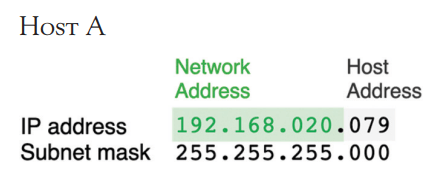
\includegraphics[width=67mm, keepaspectratio]{figures/host_a.png}
        \caption{Host A}
    \end{minipage}\hfill
    \begin{minipage}{0.45\textwidth}
        \centering
        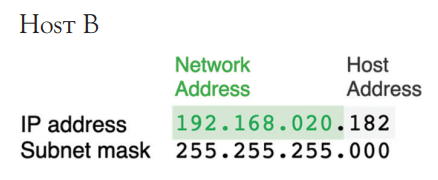
\includegraphics[width=67mm, keepaspectratio]{figures/host_b.png}
        \caption{Host B}
    \end{minipage}
\end{figure}
%----------------------------------------------------------------------------
Host A Host B  Host B ugyanabban az alhálózatban van,
mint Host A, mert mindkettő ugyanazt a hálózati címkét használja (192.168.020).
Az IP-cím hálózati része az a rész, ahol az alhálózati maszk 255-ös értéket
mutat. Ezen két eszköz között egy router sem szükséges. 
%----------------------------------------------------------------------------
\begin{figure}[H]
	\centering
	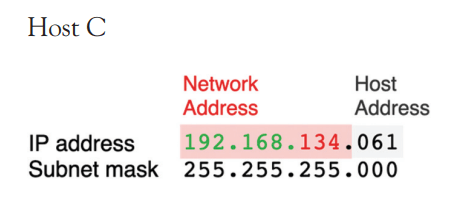
\includegraphics[width=67mm, keepaspectratio]{figures/host_c.png}
	\caption{Host C}
	\label {fig:host_c}
\end{figure}
%----------------------------------------------------------------------------
Host C más alhálózatban van, mint Host A és B, mert különbözik a hálózati címében (192.168.134, nem pedig 192.168.020).
Host C nem tud csomagokat cserélni A és B eszközökkel egy router nélkül. 
Annak érdekében, hogy ez az eszköz kommunikálhasson A és B-vel, más IP-címet kell kapnia,
kezdve a 192.168.134\ldots címmel. 
Vagy más alhálózati maszk is választható az egész beállításhoz,
például 255.255.0.0.
%----------------------------------------------------------------------------
A feljegyzett alhálózati maszkok decimális jelölése dot-decimális jelölésnek nevezik.
Azért, hogy az információt rövidebben jelezzék, gyakran
használt alternatív módszer a CIDR vagy perjeljelölés.
Az IP-cím után azonnal következő perjel után az
alhálózati maszkot a `0'-nál nagyobb értékeket mutatva jelöli meg.
Ez a jelölés az alhálózati maszk bináris formájára utal, tehát a `255' a `11111111' -nek felel meg.
A fenti példákban az alhálózati maszkok tehát bináris formájukban 24
`1'-t tartalmaznak. 
A fenti példában szereplő hosztok CIDR jelölése:

%----------------------------------------------------------------------------
\begin{itemize}
    \item \textbf{Host A:} 192.168.020.182/24
    \item \textbf{Host B:} 192.168.020.079/24
    \item \textbf{Host C:} 192.168.134.61/24
\end{itemize}
%----------------------------------------------------------------------------

A routereket használó és több alhálózatot összekapcsoló telepítések a
az OSI modell 3. rétegén működnek. Ez a modell hét rétegre osztja a
hálózatok általános funkcionalitását, mindegyik egy adott készletet ír le a hálózati
eszközök által nyújtott funkcionalitásokról. Gondolva itt elsősorban a csomagok továbbításáról a
megfelelő címzett felé. 

Az összes jelenlegi IT eszköz követi ezt a jól
meghatározott absztrakciós rétegkoncepciót, hogy elősegítse a gyártók közötti
interoperabilitást. A 3. rétegen működő telepítések értelmezhetik az IP-címeket,
az alhálózati maszkokat, és így továbbítani tudják a csomagokat az
alhálózatok között. Az itt tárgyalt összes technológia képes így működni. 
Ezzel szemben néhány technológia korlátozódott a 2.rétegre. 
Ez azt jelenti, hogy a csomagjaikat kizárólag MAC-címek alapján
szállítják, és nem tartalmaznak alhálózati információkat. Ennek eredményeként a
2. rétegű hálózatokat nem lehet több alhálózatokra bontani, a csomagjaikat nem
lehet routerek által továbbítani, és ezáltal a skálázhatóságuk korlátozott. 
Az egyik népszerű példa a 2. rétegű hálózatokra a már említett TSN/Milan, valamint a CobraNet.

%----------------------------------------------------------------------------
\begin{figure}[H]
	\centering
	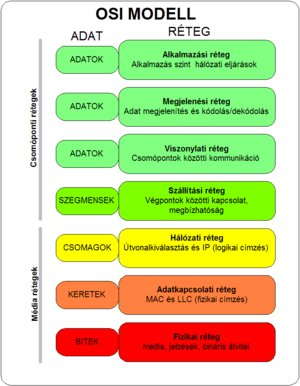
\includegraphics[width=150mm, keepaspectratio]{figures/osi_modell.jpg}
	\caption{Az OSI modell}
	\label {fig:osi_modell}
\end{figure}
%----------------------------------------------------------------------------

Egy alhálózat egy logikai szegmens egy adott hálózaton belül. Ilyen szegmenseket
különféle okokból hoznak létre, ideértve elsősorban az adminisztratív és biztonsági
szempontokat. A routerek képesek összekapcsolni az alhálózatokat, így a hosztok csomagokat cserélhetnek az
alhálózati határok átlépése nélkül. Megfelelően konfigurálva kell
lennie a hálózati útvonalak létrehozásához ezek között az alhálózatok között.
Ezzel szemben egy tipikus kapcsoló nem képes összekapcsolni az alhálózatokat.
Virtuális LAN készítése (VLAN) egy másik módszer a hálózat szegmentálására. 
Rugalmasabbá teszi a rendszereket, csökkenti a kapcsolatlan rendszerek közötti fölösleges kommunikációt.
Szemben az alhálózatokkal, ez egy biztonságosabb módja is a hosztok elkülönítésére egymástól.

%----------------------------------------------------------------------------
\subsection{Hálózati topológiák}
%----------------------------------------------------------------------------
A csomópontok különböző módon kapcsolódhatnak össze. A topológia meghatározása
az egyik legfontosabb döntés, amelyet egy hálózat tervezésekor hozni kell. A
csillag topológia sok szempontból preferált megoldás. Több hoszt egy
útválasztó eszközhöz, például egy kapcsolóhoz vagy routerhez csatlakozik. A mai
hálózatok gyakran két csillagszintet kombinálnak. Ezt gerinc/levél architektúrának
nevezik. A központi kapcsoló/router (gerinc) általában több forgalmat továbbít,
mint a perifériális kapcsoló (levél). Ha a gerinc és a levél közötti nagy sávszélességű
kapcsolat nem képes egyszerre továbbítani az összes hoszt forgalmát, akkor ez a
tervezési forma blokkoló. Az ellentéte egy nem blokkoló hálózattervezés, ahol a
nagy sávszélességű kapcsolatok képesek az összes a hozzájuk csatlakoztatott
hoszt teljes forgalmát továbbítani. A gyűrű topológiának több interfésze is lehet:
legalább kettőre van szükség egy gyűrű topológia megvalósításához. Minden két
csomópont közötti kapcsolat teljes sávszélességet kínál, és a csomópontokra
hárul a feladat, hogy továbbítsák a csomagokat a gyűrűn belül. Ebben az
értelemben mindegyik csomópont úgy működik, mint egy kapcsoló, csomagokat
továbbítva két interfésze között. A gyűrű topológia választása gyakran ésszerű,
amikor nagy távolságokat kell áthidalni, és a kapcsolatok költségesek.
Gyakorlati példák a különböző helyszínek közötti hálózatok, de gyűrűket alkotnak
olyan eszközök csatlakoztatására is, amelyek esetében nincs hely egy további
kapcsoló számára. A gyűrű topológiák beépített redundanciát kínálnak minden
eszközhöz hozzáférhetünk, még akkor is, ha egy kapcsolat elszakad.
A megfelelő hálózat kialakításához még elengedhetetlenek a nem blokkoló kapcsolók.
A nem blokkoló architektúra azt jelenti, hogy nem a kapcsoló a szűk keresztmetszet.
Tehát képes kezelni az összes rá táplált forgalmat, csak a port sebessége a korlát.

%----------------------------------------------------------------------------
\subsection{Unicast és Multicast} %Egyedi és Csoportos Küldés
%----------------------------------------------------------------------------

Amikor egy eszköz csomagot küld egy másik eszköznek, unicast mechanizmusnak
nevezzük. Egy ilyen kapcsolatnak pontosan egy küldője és egy fogadója van. Az
unicast gyakran használja a Transmission Control Protocol (TCP)-t, ahol a fogadó
minden egyes csomag sikerült átvételéről visszaigazolást küld a küldőnek. Ha a
visszaigazolás nem érkezik meg, a küldő automatikusan újraküldi a csomagot. 
Az UDP (User Datagram Protocol) egy alternatíva a TCP-nek. Ebben az esetben a küldő
bízik abban, hogy a csomagok sikeresen megérkeznek a fogadóhoz. Nincs
visszaigazolás, és ha a csomag elveszik, a tartalma is elveszik.
Ez az jelenti, hogy az UDP nem annyira megbízható? Valójában nem,
csak egy más eszköz más felhasználásra.
Bár ez váratlan lehet, ez valójában a preferált átviteli mód a szakmai audio hálózatok
számára. Mivel az időkésleltetés alacsonynak kell lennie, nem engedhető meg a
csomagok újraküldése, mert az időt vesz igénybe, és ezzel növelné az általános
időkésleltetést. Az élő audio csomagvesztés esetén a legjobb, ha folytatjuk a
következő audio minták lejátszását, anélkül hogy megpróbálnánk helyreállítani az
előzőt. A menedzselhető switchek és végpontok tudják logolni a csomagvesztéseket, így
monitorozható a hálózat állapota.
Az audio alkalmazásokban gyakran szükség van arra, hogy egy audio jelet
több helyen párhuzamosan fogadjanak, például egy mikrofonjel, amelyet
párhuzamosan továbbítanak a front-of-house és a monitoring keverőpultoknak. Akár
egy harmadik hely is létezhet, például egy felvevő eszköz. 
Amikor a küldő unicast módban továbbítja a csomagokat, az audio jel három csomagként
érkezik azonos tartalommal, de különböző címzési címekkel. Ez felesleges
processzor terhelést jelent a küldő eszköz számára, és emellett sávszélességet
foglal el mindhárom célhoz. Ezt lehet optimalizálni a multicast használatával. 
Számos előnye van, ideértve a küldőre nehezedő kevesebb processzor terhelést 
és az általános forgalom csökkenését a hálózaton. 
A küldő multicast címekre címezi a csomagokat, és nem hoszt címekre. Nem tudja, melyik
címzetteknek érkeznek meg a csomagok. A multicast címek hasonlóak a
rádiófrekvenciákhoz: bárki, aki érdeklődik, bekapcsolhatja és fogadhatja a
tartalmat. A küldő csak egyszer helyezi az audio adatokat egy csomagba, elküldi
egy multicast címre, és a vevőknek tudniuk kell, melyik multicast címre akarnak
hallgatni. A multicast címek alapvetően nem kapcsolódnak alhálózatokhoz, mivel nem
kapcsolódnak a csomópontokhoz és az IP-címekhez. Ezért a multicast csomagok
áthaladnak az alhálózatokon, hacsak nincsenek elkülönítve VLAN-okkal. 
Amennyiben a hálózatunk nem kizárólag az audio jelek továbbítására 
készült speciálisan, néhány eszköz lehet a hálózaton, amelyeknek semmi közük az audiohoz.
Ezért fontos, hogy a multicast forgalom csak
azokhoz a hosztokhoz jusson el, amelyek érdeklődnek iránta. Ennek a megoldása az
IGMP snooping (Internet Csoportkezelési Protokoll). 
Az összes tárgyalt audio hálózati technológia alapértelmezetten
támogatja az IGMP snooping-ot. Ha be van kapcsolva a kapcsolóban, akkor a
multicast-csomagok csak azokon az interfészeken kerülnek elküldésre, ahol a
csatlakoztatott hosztoktól időszakos IGMP kérések érkeznek. Ha nincs beérkező
kérés, akkor a megfelelő multicast leáll, így nem jut felesleges forgalom a
kapcsolatra. Az IGMP snoopingot egyfajta zsilippel lehetne összehasonlítani,
amely alapértelmezetten zárva van, és csak kérésre nyílik meg. Erősen ajánlott
az IGMP snooping bekapcsolása egy multicast hálózatban minden kapcsolóban.
Azonban egy hálózatban csak egy darab IGMP Querier lehet aktív, mivel az
összes többi kapcsoló az aktív IGMP Querier-től kapja az információkat.
Enélkül a multicast úgy viselkedni mint egy broadcast, ami nagy mennyiségű
felesleges forgalmat eredményez.
Összefoglalva, a unicast a legjobb késleltetési teljesítményt nyújtja, és a
kapcsolók számára a legkönnyebben mozgatható.
A multicast pedig jobb sávszélesség-kezelést kínál, ahogy a csatornaszám (és a sávszélesség) nő.

%----------------------------------------------------------------------------
\subsection{Eszköz- és Adatfolyam-felfedezés}
%----------------------------------------------------------------------------

Az AES67 audió szabvány nem határozza meg, hogyan fedezhetik fel egymást a
hálózati eszközök, vagy hogy mely adatfolyamok érhetők el a hálózaton.
Az összes ismert technológia a bonjour vagy mDNS mechanizmust használja eszközeik számára
az egymásról való értesítésre. 
Minden eszköz fix ismert multicast cím (224.0.0.251) felé küld
üzeneteket, amiket más eszközök elérnek, így értesülnek egymás létezéséről a hálózatban.
Ennek a mechanizmusnak egyik korlátja az, hogy nem működik nagy telepítésekben,
ahol több alcím létezik vagy VLAN-on vannak. Ezen esetekre a gyártók kifejlesztettek
saját megoldásokat (például Audinate a Dante Domain Manager) vagy
követik az audio/video NMOS szabványt a felismeréshez és kapcsolatkezeléshez.
Az audio adatfolyamokat a gyártótól függően két mechanizmus egyikével fedezik fel. Ahogy
az eszközök felfedezésénél, mindkettő előre meghatározott multicast címet
használ az adatfolyam-információk terjesztésére, hogy a címzettek megtalálják az
elérhető adatfolyamokat és azok paramétereit:

%----------------------------------------------------------------------------
\begin{itemize}
	\item Session Announcement Protocol (SAP) - minden Dante termék által használt (Multicast cím: 239.255.255.255)
\end{itemize}

\begin{itemize}
	\item Bonjour / mDNS - minden más technológiában használt (Multicast cím: 224.0.0.251) 
\end{itemize}
%----------------------------------------------------------------------------
Szerencsére a jelenlegi termékek többsége
lehetővé teszi mindkét protokoll egyidejű aktiválását, így egy adott audio
adatfolyam mindkét mechanizmuson keresztül párhuzamosan bejelenthető.

%----------------------------------------------------------------------------
\subsection{Redundancia}
%----------------------------------------------------------------------------
Az audiohálózatok kezdeti napjaiban egyes felhasználók kételkedtek az IT
hardverek megbízhatóságában. Annak ellenére, hogy a széles körben elterjedt
IT-berendezések jól beváltak és gyakran megbízhatóbbak, mint a hagyományos
audioberendezések. Emellett a legtöbb IT-hálózati komponens több diagnosztikai
mechanizmust kínál a berendezések hibájának gyors felismeréséhez és megoldásához.

%----------------------------------------------------------------------------
\subsubsection{Spanning Tree Protocol (STP)}
%----------------------------------------------------------------------------
Ha a kapcsolókat úgy kötik össze, hogy hurok jön létre, fennáll annak a veszélye, 
hogy a csomagok végtelenül áramlanak a hurokban. 
Ezt az `visszacsatoló hurok' jelenséget a hálózati hardver automatikusan észleli az
STP segítségével, és ha hurokra bukkan, a kapcsoló automatikusan kikapcsolja az egyik
kapcsolatot. Az STP-t viszont felhasználhatják a rendszer véletlen
kapcsolatvesztések elleni védelmére is, beleértve a kábelvágásokat is. 

Abból a  megközelítésből áll, hogy szándékosan létrehoznak hurkokat, majd a rendszer
inaktiválja az egyiket, ha valamelyik kábel véletlenül kiesik, a rendszer
másodperceken belül észleli ezt, és újraaktiválja a passzív kapcsolatot. Ebben
az időszakban az audio néhány másodpercig megszakad, de még mindig sokkal
gyorsabb, mint a manuális hibakeresés és az új kábel telepítése. 
A legtöbb rendszerben az STP alapértelmezetten engedélyezve van. 
Nélküle broadcast 'viharok' alakulnának ki, ami felemészti a sávszélességet, és túlterheli a hálózatot.

%----------------------------------------------------------------------------
\subsubsection{Link Aggregáció}
%----------------------------------------------------------------------------
Ha egy adott kapcsolat különösen fontos egy telepítésben, két vagy több kábelt párhuzamosan
lehet csatlakoztatni a biztonság érdekében. 
Bár az ilyen link aggregáció fő célja két kapcsoló közötti sávszélesség növelése. 
Ez is költséghatékony módszer lehet egy kapcsolat véletlen leválasztásának
vagy kábelvágásának biztosítására. Tipikus eset például egy színpad, amely egy keverőhöz
csatlakozik. A kapcsolóknak mindkét végén ugyanúgy kell konfigurálni: két vagy
több interfészt kell kijelölni Link Aggregációs Csoportként, és azok
egyetlen interfészként jelennek meg a kapcsolón. Gyakorlatban a linkaggregáció
alkalmazása a kábelproblémák csökkentése érdekében nagyon hasznos lehet.
Egyszerűsége miatt, a felhasználónak csak egy további kábelt kell
biztosítania, és azonosítania kell a kapcsolók konfigurációját mindkét végén.
Ugyanakkor a kábelt lekapcsoláskor előfordulhat, hogy az audioátvitel
néhány másodpercig itt is megszakad, mielőtt a kapcsoló alternatív kapcsolatot
aktiválna.
%----------------------------------------------------------------------------
\subsubsection{ Adatfolyam redundancia}
%----------------------------------------------------------------------------
A legbiztonságosabb de egyben legdrágább módja a redundancia megvalósításának
egy hálózatban az, ha két különálló audiohálózatot hoznak létre, 
két független utat biztosítva a küldő és a fogadó között. 
Ebben a felállásban minden csomópontnak két hálózati interfészt
kell biztosítania. A küldő két azonos audio tartalommal rendelkező csomagot hoz létre,
mindkettőre azonos PTP-időbélyegzőt nyom, majd elküldi mindkét hálózaton.
A fogadó végén mindkét csomagot fogadják és kicsomagolják. Még akkor is, ha az egyik csomag
elveszik, a megmaradt csomag tartalmazza az összes információt, és biztosítja,
hogy az audio zavartalanul folytatódik. Valójában ez a mechanizmus az egyetlen
megközelítés egy hálózatban a véletlenszerű csomagvesztés kompenzálására anélkül,
hogy meg kellene ismételni azokat a küldőtől és ezzel késleltetést hozzáadva a rendszerhez.
%----------------------------------------------------------------------------
\section{AES67}
%----------------------------------------------------------------------------
Az AES67 szabvány szerint az összes eszköznek meg kell felelnie az
alábbi minimális specifikációknak: 

%----------------------------------------------------------------------------
\begin{itemize}
	\item Unicast és multicast támogatása
	\item UDP/RTP protokollok használata
	\item DSCP címkék beállítása meghatározott értékekre,QoS támogatás 
	\item Nincs meghatározott automatikus eszköz- és adatfolyam-felfedezés 
	\item PTPv2 szabvány használata az időszinkronizációhoz
	\item PTP profil Standard (a gyakorlatban a Dante jelenleg magasabb szinkronizációs rátát igényel)
	\item Küldőknek ki kell adniuk egy SDP fájlt
	\item A fogadóknak érteniük kell egy SDP fájlt
	\item A fogadó puffernek legalább 3 ms hangot kell tudnia tárolni
	\item Adatfolyam formátumok
	\item Egytől nyolc csatorna (a küldő választhat egy fix számot, de a fogadóknak képesnek kell lenniük rugalmasan fogadni bármelyik lehetőséget).
	\item 24 bites és 16 bites felbontás (a küldő választhat egyet, de a fogadóknak mindkettőt érteniük kell) 
	\item 48 kHz mintavételi frekvencia 1 ms csomagidő (48 minta)
	\item A multicast címek 239.0.0.0 és 239.255.255.255 között vannak 
\end{itemize}

A szabványban sok további paraméter és érték szerepel, de ezek nem szerepelnek a
fent felsorolt minimális követelmények között.

%----------------------------------------------------------------------------
\section{Audinate Dante}
%----------------------------------------------------------------------------
\subsection{A Dante hálózatok áttekintése}
%----------------------------------------------------------------------------
A 2020 - 2021-es Covid-19 járvány alatt lehetőségem volt egy széleskörű Dante
kurzusra beiratkozni, amelyet a Dante gyártója, az Audinate szervezett. A kurzus
egy átfogó mély áttekintést nyújtott a Dante hálózatokról. Ebben a fejezetben
fő forrásomnak a belsős oktatóanyagot fogom használni, amelyet a kurzus
során kaptam, pontos és részletes információkat nyújtva a Dante hálózatokról.
Ezek a dokumentumok csak azok számára elérhetőek, akik részt vettek a kurzuson, ebből kifolyólag nem publikusak.

A Dante hanghálózatok digitális hanghálózati technológiát képviselnek, amely
lehetővé teszi a hang elosztását és útválasztását a szabványos Ethernet
hálózatokon keresztül. Az ausztrál Audinate vállalat fejlesztette ki a Dante-t,
amely a szabványos Internet Protocol (IP) hálózatokat használja a magas minőségű,
alacsony késleltetésű hangátvitelhez eszközök között. Ez lehetővé tesz
nagyobb rugalmasságot és skálázhatóságot a hagyományos analóg hangrendszerekhez
képest, valamint biztosítja a hangrendszer integrálását egy meglévő IT infrastruktúrába.
A Dante hanghálózatokat széles körben alkalmazzák, ideértve a koncerthangosítást,
rádiózást, stúdiófelvételeket, vállalati és konferenciaközpontokat, és még sok mást.
A technológia támogat számos hangformátumot és mintavételi rátát, és lehetővé
teszi akár több száz hangcsatorna egyidejű átvitelét egyetlen hálózaton keresztül.
Emellett a Dante hanghálózatok távolról is vezérelhetők és monitorozhatók,
megkönnyítve a nagy, összetett hangrendszerek beállítását és kezelését.

%----------------------------------------------------------------------------
\subsection{Dante hálózatok technikai részletei}
%----------------------------------------------------------------------------
A Dante hanghálózatok két fő komponensből állnak: Dante eszközökből
és Dante hálózatokból. A Dante eszközök olyan hangeszközök, amelyeket
kifejezetten a Dante protokollhoz terveztek, mint például hangkártyák, erősítők
és hangládák. Ezeket az eszközöket szabványos Ethernet kábelekkel és
kapcsolókkal lehet csatlakoztatni a Dante hálózathoz.
A hálózatot az Audinate Dante Controller szoftverrel lehet
konfigurálni, amely lehetővé teszi a hang elosztását és útválasztását az
eszközök között. A szoftverrel tudjuk az eszközöket távoli vezérléssel elérni és
monitorozni a hálózaton. Ezek a hanghálózatok támogatnak számos
hangformátumot és mintavételi rátát, és képesek egyszerre több száz hangcsatorna
átvitelére egyetlen hálózaton keresztül. A technológia továbbá támogat olyan
fejlett funkciókat, mint a Dante Domain Manager (DDM) a biztonságos
hangátvitelhez, valamint a Dante Virtual Soundcard (DVS) a számítógépes alapú
hanglejátszáshoz és felvételhez. 

Tegyük fel, hogy több eszköz is küld hangot egy adott végpontra a hálózaton.
Alapesetben, ahogy a csomagok felgyülemlenek, az elsőként érkezőket, elsőként szolgálják ki elvet alkalmazzák.
A Dante hanghálózatok Quality of Service (QoS)
támogatást is nyújtanak, a prioritások kezelésére.
Ezzel biztosítható a hangátvitel elsőbbse más hálózati forgalommal szemben. Ez segít minimalizálni a hálózati
torlódás lehetőségét és biztosítani, hogy a hangátvitel minimális késleltetéssel
és magas minőségben történjen. 
Körülbelül 70 százalékos hálózati szaturációnál már ajánlott a QoS használata.
Valamint 100 Mbps-es hálózatoknál segít a jitter csökkenésében.

%----------------------------------------------------------------------------
\subsubsection{Több mintavételi ráta és bitmélység}
%----------------------------------------------------------------------------

A rendszer képes egyidejűleg több bitmélységet kezelni. Ennek informatikai háttere a
a következő képpen néz ki. Ha egy 32 bites hangforrásunk van, de a másik eszköz
csak 24 bites hangot tud fogadni, akkor a Dante a 32 bites hangot 24 bitesre tudja 
alakítani.

%----------------------------------------------------------------------------
\begin{align*}
	\begin{array}{|c|c|}
	\hline
	\text{Hangminták} & \text{Bitmélység} \\
	\hline
	\text{11110000 11110000 11110000 11110000} & \text{32 bites} \\
	\hline
	\text{11110000 11110000 11110000} & \text{24 bites} \\
	\hline
	\end{array}
\end{align*}
%----------------------------------------------------------------------------
	
Amint a példában látszik, 32 bites hangból úgy kaptunk 24 bites hangot, 
hogy egyszerűen csak elhagytuk az utolsó 8 bitet. Ez a folyamat visszafelé is működik,
ha 24 bites hangot kell 32 bites hanggá alakítani, akkor az utolsó 8 bitet 0-val kell feltölteni.

%----------------------------------------------------------------------------	
\begin{align*}
	\begin{array}{|c|c|}
	\hline
	\text{Hangminták} & \text{Bitmélység} \\
	\hline
	\text{11110000 11110000 11110000} & \text{24 bites} \\
	\hline
	\text{11110000 11110000 11110000 00000000} & \text{32 bites} \\
	\hline
	\end{array}
\end{align*}
%----------------------------------------------------------------------------

Mintavételezési frekvencia eltérést csak abban az esetben tudja kezelni, ha a
bitmélység is eltérő. Amennyiben a bitmélység azonos, de a mintavételezési
frekvencia eltérő, akkor a rendszer nem képes a hangot továbbítani.
Ez a mechanizmus egy egyszerű mechanikai példával jól megérhető és leírható.
Tegyük fel van két fogaskerekünk. Amennyiben a mintavételezési frekvencia azonos, és a 
bitmélység eltérő, akkor a fogaskerekek egymásba illeszthetőek és csak a fogaskerekek
mélysége fog eltérni. Amennyiben a mintavételezési frekvencia eltérő, akkor a fogaskerekek
nem illeszthetőek egymásba, és nem tudjuk továbbítani a hangot. Ebben az esetben már egy
konverterre lesz szükségünk, amely képes a két fogaskereket összeilleszteni számunkra.
Egy fontos kitétel van ahhoz, hogy a több mintavételi ráta egyszerre megfelelően működjön,
az pedig az egységes órajel az összes mintavételi frekvenciához.

%----------------------------------------------------------------------------
\subsubsection{Hálózati topológiák}
%----------------------------------------------------------------------------
A Dante rendszerek alapvetően kétféle módban tudnak üzemelni. Az első a
switched (kapcsolt) mód, amelyben az eszközökön található két Ethernet port
egy hálózatot alkot. Ebben a módban tudunk Daisy Chain (füzéres) topológiát kialakítani,
amelyben az egyik eszköz a másikhoz csatlakozik, és így tovább. Továbbá csillagtopológiát
is kialakíthatunk, amelyben minden eszköz egy központi kapcsolóhoz csatlakozik.
%----------------------------------------------------------------------------
\begin{figure}[H]
	\begin{minipage}{0.5\textwidth}
		\centering
		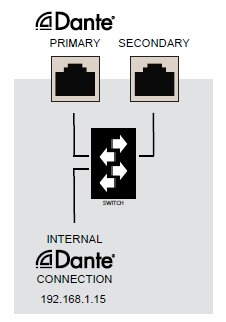
\includegraphics[width=100px, keepaspectratio]{figures/dante-switched-mode.jpg}
		\caption{Kapcsolt mód}
		\label{fig:dante_switched}
	\end{minipage}%
	\begin{minipage}{0.5\textwidth}
		\centering
		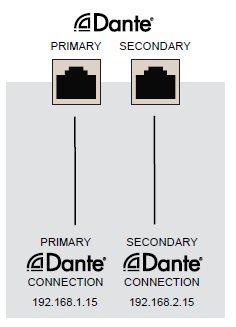
\includegraphics[width=100px, keepaspectratio]{figures/dante-redundant-mode.jpg}
		\caption{Redundáns mód}
		\label{fig:dante_redundant}
	\end{minipage}
\end{figure}

%----------------------------------------------------------------------------
A másik mód a redundant (redundáns) mód, amelyben az eszközökön található két
Ethernet port két különálló hálózatot alkot. Ebben a módban a hálózat redundáns
kialakítású, és a hálózat egyik része automatikusan átveszi a másik rész szerepét,
ha az meghibásodik.
Néhány Dante eszköznek létezik egy harmadik Ethernet portja, amelyet konfigurálási
és vezérlési célokra használnak.
%----------------------------------------------------------------------------
\subsubsection{Késleltetés}
%----------------------------------------------------------------------------
A késleltetés az az idő, amely szükséges egy folyamat végrehajtásához. Például
az idő amíg a bemeneti oldalon egy hangjel feldolgozásra kerül, és a kimeneti
oldalon megjelenik. 
Két fő mértékegységet használunk a késleltetés mérésére:
%----------------------------------------------------------------------------
\begin{equation}
	\label{eq:milliseconds}
	1 \text{ másodperc} = 1000 \text{ milli másodperc}, \quad \text{azaz} \quad 1 \text{ ms} = 0.001 \text{ s}
\end{equation}
%----------------------------------------------------------------------------
%----------------------------------------------------------------------------
\begin{equation}
	\label{eq:microseconds}
	1 \text{ másodperc} = 1000000 \text{ mikro másodperc}, \quad \text{azaz} \quad 1 \mu\text{s} = 0.000001 \text{ s}
\end{equation}
%----------------------------------------------------------------------------
A Dante eszközök lehetővé teszik a késleltetés teljesítményének meghatározását. 
A 0.1 milliszekundumos késleltetés az a késleltetés, amely már kapcsoló lépés biztos.
Ha két eszköz különböző késleltetésű, akkor a nagyobb érték lesz az irányadó.
Egy megfelelően konfigurált modern Dante hálózatban a késleltetés 1 ms körüli értéket vesz fel.
Ez azt is jelenti, hogy például egy dobos előbb hallja a hangszerét a fülmonitoron, mint a saját dobját.

%----------------------------------------------------------------------------
\subsubsection{Órajel}
%----------------------------------------------------------------------------

Minden eszköz egy nagyon-nagyon pontos Dátum/Idő órát követ.
Szinkronizálnak az időhöz és állítják a sebességet, hogy egységes legyen.
Mi a helyzet a terjedési késéssel? Miért vannak szinkronban a Dante eszközök?
A PTP (Precision Time Protocol) késleltetési kéréseket (Delay Requests)
ad ki, amelyek kiszámítják a hálózat késleltetését. 
Az eszközök az információváltás késését is kompenzálják.
A Dante automatikusan választ óra vezetőt.
Mindig csak egy óra vezető lesz, függetlenül a mintavételi rátától.
Beállíthatunk külső óra vezetőt is amennyiben szükséges.
Nem szinkronizál újra, hanem beállítja a sebességet és kompenzálja a hálózati késést.
A Dante által végzett tesztelések és tapasztalatok alapján
bebizonyosodott, hogy az időzítés szinkronban marad akkor is,
ha az óra perceken keresztül teljesen eltűnik.

%----------------------------------------------------------------------------
\begin{figure}[H]
	\centering
	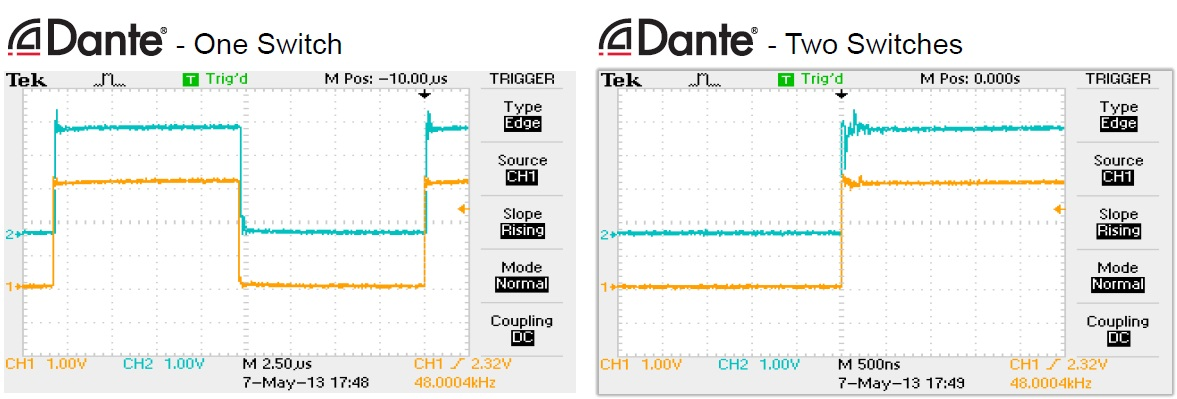
\includegraphics[width=400px, keepaspectratio] {figures/dante-clocking.jpg}
	\caption{Dante órajel}
	\label{fig:dante-clock}
\end{figure}
%----------------------------------------------------------------------------

%----------------------------------------------------------------------------
\subsection{Összehasonlítás a hagyományos hangrendszerekkel}
%----------------------------------------------------------------------------
A hagyományos hangrendszerek általában analóg kábelekre és csatlakozókra
támaszkodnak a hangjelek eszközök közötti átviteléhez. Ezek a rendszerek
korlátozottak lehetnek rugalmasságban, skálázhatóságban és az egyidejűleg
átvihető hangcsatornák számában. Emellett hajlamosak bonyolultabbá válni a
beállítás és kezelés szempontjából, mivel minden hangcsatornához külön kábel és
csatlakozás szükséges. A Dante hanghálózatok jóval több hangcsatornát is támogatnak,
mint a hagyományos analóg rendszerek, lehetővé téve a nagy, összetett hangrendszerek könnyű
beállítását és kezelését. A Dante hanghálózatok további előnye, hogy képesek
hangot továbbítani hosszú távolságokon anélkül, hogy a minőség romlana. A
hagyományos analóg rendszerek zajra és jelveszteségre hajlamosak hosszú kábelek
esetén, míg a digitális hangjelek, amelyeket az Ethernet hálózatokon
továbbítanak, minimális minőségveszteséggel juthatnak el nagy távolságokra.
%----------------------------------------------------------------------------
\begin{table}[htbp]
    \centering
    \caption{Digital Snake és DigitalAVNetwork Jelút opciók}
    \begin{tabular}{@{}lll@{}}
        \toprule
        \textbf{Kérdés} & \textbf{Pont-pont között} & \textbf{Hálózati megoldás} \\ \midrule
        Hová megy a jel? & Lineáris kábelút & Bárhol a hálózaton \\
        Hogyan változtassuk meg a jelútvonalat? & Mozgassuk a kábelt & Egy egérkattintással \\
        Szétválaszthatjuk-e a jeleket? & Nem & Igen - a hálózaton \\
        Megosztható-e a kábel más jelekkel? & Nem & Igen - közös infrastruktúra \\
        \bottomrule
    \end{tabular}
    \label{tab:digital-snake-vs-digitalavnetwork-hu}
\end{table}
%----------------------------------------------------------------------------
\begin{figure}[H]
	\centering
	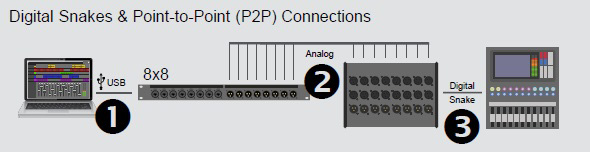
\includegraphics[width=\linewidth, keepaspectratio]{figures/dsnake-p2p.jpg}
	\caption{Digital Snake és Pont-pont közötti (P2P) kapcsolatok}
	\label {fig:dsnake-p2p}
\end{figure}
%----------------------------------------------------------------------------
\begin{figure}[H]
	\centering
	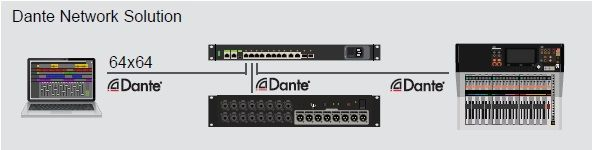
\includegraphics[width=\linewidth, keepaspectratio]{figures/dante-solution.jpg}
	\caption{Dante hálózati megoldás}
	\label {fig:dante-solution}
\end{figure}
%----------------------------------------------------------------------------

A rugalmasság és a skálázhatóság tovbbi kulcsfontosságú előnye a Dante
hanghálózatoknak a hagyományos analóg hangrendszerekkel szemben.
Képesek alkalmazkodni különböző hangkonfigurációkhoz és követelményekhez. 
Könnyű eszközöket hozzáadni vagy eltávolítani, megváltoztatni a hangjelek útvonalát, és a rendszert újra
konfigurálni szükség esetén. Ez lehetővé teszi testreszabott audio-megoldások
létrehozását, amelyeket az adott alkalmazás vagy környezet speciális igényeihez
lehet igazítani. 

%----------------------------------------------------------------------------
\subsection{Firmware frissítés}
%----------------------------------------------------------------------------

A Dante eszközök rendelkeznek Dante Firmware és Eszköz Firmware-el.
Lehet, hogy mindkettőt frissíteni kell. Kérjük, forduljon a gyártóhoz a párosított verziókért.
Néhány eszköz sorozat más módszerekkel frissíthető.
A Dante Updater hasznos lehet a frissítések nyomon követéséhez és telepítéséhez.
A rendszer ellenőrzi az online adatbázisunkat, hogy tájékoztassa Önt az elérhető frissítésekről.
A Dante firmware könnyen frissíthető.
A Dante Firmware Update Manager továbbra is aktuális.
Importálja a firmware fájlokat, ha firmware-t kap egy gyártótól.
Ha a frissítés nem sikerül, rendelkezünk vészhelyzeti helyreállítási módszerrel.
A Dante eszközök erős támogatást nyújtanak a vegyes firmware verziókhoz.
Mérnökeink automatizált regressziós tesztelést végeztek a korábbi firmware kiadásokkal szemben.

%----------------------------------------------------------------------------
\subsection{Chipek}
%----------------------------------------------------------------------------

A Dante hálózatok változatos chipekkel építhetők fel. 
Az Audinate számos különböző chipet kínál a Dante hálózatok létrehozásához, 
melyek eltérő hangcsatorna-számot és egyéb funkciókat támogatnak. 
A Dante chipek különféle méretekben és árkategóriákban elérhetők, 
lehetővé téve a gyártók számára, hogy különféle méretű és árú Dante 
eszközöket fejlesszenek ki, így képesek kielégíteni a különböző piaci igényeket. 
A Dante chipek segítik a gyártókat abban, hogy gyorsan és hatékonyan hozzanak 
létre Dante-kompatibilis eszközöket, és könnyedén integrálják azokat a saját termékeikbe.

%----------------------------------------------------------------------------
\begin{center}
	\begin{tabular}{|c|p{10cm}|}
		\hline
		\textbf{Chip} & \textbf{Leírás} \\
		\hline
		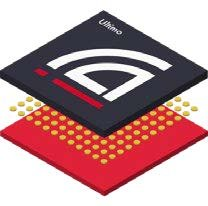
\includegraphics[width=40px,height=40px,keepaspectratio]{figures/ultimo-x.jpg} & \textbf{Dante Ultimo-X} - 0x4, 2x2, 4x0 \\
		\hline
		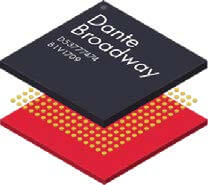
\includegraphics[width=40px,height=40px,keepaspectratio]{figures/broadway.jpg} & \textbf{Dante Broadway} - 16x16 \\
		\hline
		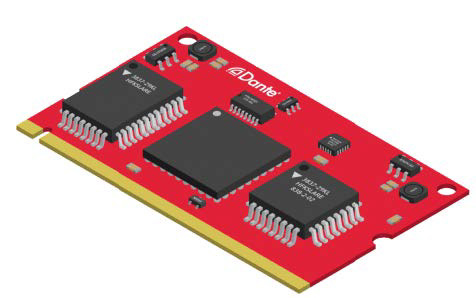
\includegraphics[width=40px,height=40px,keepaspectratio]{figures/brooklyn-ii.jpg} & \textbf{Dante Brooklyn II} - 64x64 \\
		\hline
		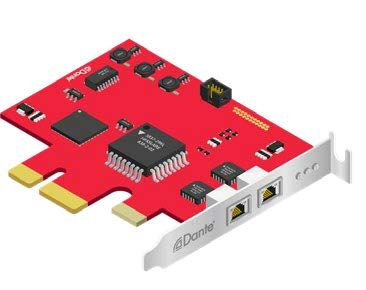
\includegraphics[width=40px,height=40px,keepaspectratio]{figures/pcie-r.jpg} & \textbf{Dante PCIe-R} - 128x128 \\
		\hline
		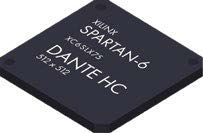
\includegraphics[width=40px,height=40px,keepaspectratio]{figures/dante-hc.jpg} & \textbf{Dante HC (High Capacity)} - 512x512 \\
		\hline
		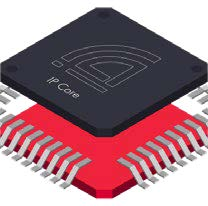
\includegraphics[width=40px,height=40px,keepaspectratio]{figures/shared-processor.jpg} & \textbf{Dante Shared Processor} - IP Core 512x512 FPGA and Dante Embedded Platform 64x64 X86/ARM \\
		\hline
		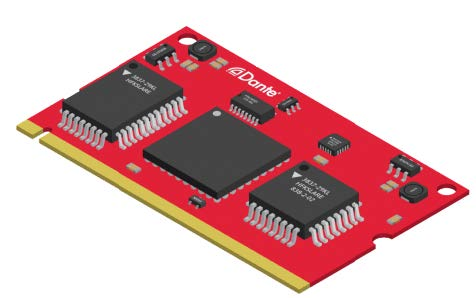
\includegraphics[width=40px,height=40px,keepaspectratio]{figures/dante-av.jpg} & \textbf{Dante AV} - V:1, A:8 \\
		\hline
	\end{tabular}
\end{center}
%----------------------------------------------------------------------------
	






